\documentclass[journal, letterpaper]{IEEEtran}
%\documentclass{scrartcl}

\usepackage[ngerman,english]{babel}
%\usepackage[latin1]{inputenc}
\usepackage[utf8]{inputenc}
\usepackage[T1]{fontenc}
\usepackage{amsmath}
\usepackage{amsthm}
\usepackage{amsfonts}
\usepackage{tikz}
\usepackage{verbatim}
\usepackage{subcaption}
\usepackage{algorithm}
\usepackage{algorithmic}
\usepackage[pdftex]{hyperref}

\renewcommand{\algorithmicrequire}{\textbf{Input:}}
\renewcommand{\algorithmiccomment}[1]{\ \ // #1} % C-like // Comments

\hyphenation{render}

\begin{document}

%\title{Simulating elastic spheres without external forces}
%\subtitle{Project 1 for class CS6491 Computer Graphics}
\title{Cube with Spheres \\
	{\large Project 1 for class CS6491 Computer Graphics}}
%\author{Sebastian Weiss}
\author{Sebastian Weiss \\ \today}
%\date{\today}

\maketitle

\begin{tikzpicture}[remember picture,overlay]
   \node[anchor=north east,inner sep=0pt] at (current page.north east)
              {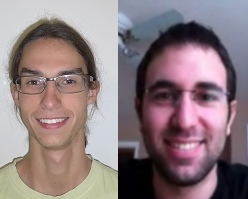
\includegraphics[scale=1.5]{pic}};
\end{tikzpicture}

\section{Objective}
In this project, we want to simulate the physically correct motion of a large number of completely elastic spheres flying around in a cube.

\section{Input}
The input consists of the following data: the initial positions and velocities of $n$ spheres and the half side length of the surrounding cube $s$.
We assume that the spheres all have the same radius $r$, the same finite mass, are constantly moving (i.e. no external forces like gravity are applied), that all collisions are completely elastic and at least one velocity is not zero. Furthermore, the spheres do not overlap with each other or the surrounding cube, but they can touch. The surrounding cube is assumed to be of infinite mass, centered at the origin of the coordinate system and aligned to the coordinate axes.

\section{Overview}
The expected bottleneck of the simulation is the physics calculation. We therefore present a framework for calculating the next collision events in parallel. 
The computation process, called the physics thread, does not check for collisions in discrete time steps, it instead computes the exact time until the next collision happens. The collision events are buffered and sent to the render thread. This thread then retrieves the collision events and draws the state of the simulation in discrete frames.

\section{Implementation}
In the following section, we present the steps needed to implement the simulation.

\subsection{Datastructures}
The sphere $i$, indexed from $0$ to $n-1$, consists of the following data: the initial position $A_i$ and velocity $V_i$ and the start time $t_i$, set to zero at the start of the simulation.

The state of the simulation consists of the following data: the current time $t_\text{global}$, initialized with 0, and an array of all spheres $S$.

A collision event $e$ contains the time of collision $t_e$ and an array with the indices of the modified spheres and their new positions and velocities at this time. It is written as $(t_e, \{(i, A_i, V_i) | \forall \text{ changed } i\})$.

\subsection{Collision computations}
This section provides the basic functions needed to compute the collision times and new velocities.

\subsubsection{Sphere-Sphere collision}\label{SSC}
Given: the spheres $i$ and $j$, and the sphere radius $r$.
A collision at time $t$ happens if $\left|(A_i + tV_i)(A_j+tV_j)\right|=2r$ is valid. Expansion leads to the following formula:
\begin{equation*}
t^2\underbrace{\left|V_i-V_j\right|^2}_{=:a} + t\cdot\underbrace{2((A_iA_j) \bullet (V_j-V_i))}_{=:b} + \underbrace{\left|A_iA_j\right|^2 - 4r^2}_{=:c} = 0
\label{eq:SSC}
\end{equation*}
This equation is then solved with $t_{1,2}=\frac{-b \pm \sqrt{b^2-4ac}}{2a}$. W.l.o.g. $t_1<t_2$. The following cases have to be distinguished:
\begin{itemize}
	\item $a=0$: the velocities of the spheres are equal, they either always intersect, always touch or always fly in parallel. So no collision is detected.
	\item $b^2-4ac < 0$: no collision detected, the spheres pass each other.
	\item $b^2-4ac = 0$: the spheres touch exactly once, no force is applied to the spheres.
	\item $b^2-4ac > 0$: the equation has two solutions, $t_1$ indicates the start of the intersection and $t_2$ the end. Only collisions with $t_1\geq 0$ are valid collisions and $t_1$ is the resulting collision time.
\end{itemize}

\subsubsection{Sphere-Sphere velocity change}\label{SSV}
Given: the spheres $i$ and $j$, and the time of collision $t$. Output: the new velocities $V'_i$ and $V'_j$ after collision.

Let $N:=(A_i+tV_i)(A_j+tV_j)$. The following formula computes the new velocities:
\begin{equation*}
V'_i=V_j \angle N - V_i \angle N + V_i \ , \ 
V'_j=V_i \angle N - V_j \angle N + V_j
\label{eq:SSV}
\end{equation*}

\subsubsection{Sphere-Cube collision}\label{SCC}
Given: the sphere $i$, the radius $r$ and the half side length $s$ of the surrounding cube. The sphere collides at time $t_{x1}$ with the lower face of the cube in x-direction, and at $t_{x2}$ with the upper face, similar $t_{y1}$ to $t_{z2}$. They are computed according to the following formula:
\begin{equation*}
t_{c1}=\frac{-s+r-A_i.c}{V_i.c} \ , \ t_{c2}=\frac{s-r-A_i.c}{V_i.c} \ \forall c\in \{x,y,z\}
\label{eq:SCC}
\end{equation*}

\subsubsection{Sphere-Cube velocity change}\label{SCV}
Since the surrounding cube is aligned to the coordinate axes, the change in velocity becomes trivial. If a sphere hits one of the two cube faces in x-direction, the x-component of the velocity is negated, and similar with the y- and z-direction.

\subsection{Multithreading and synchronization}
There exists two threads that run in parallel: the render thread and the physics thread, forming a producer-consumer pattern. The physics thread sends collision events to the render thread over a queue (e.g. a java.util.concurrent.BlockingQueue). We recommend to cap the capacity of the queue to limit the count of events that are precomputed.

\subsection{Render thread}
The render thread stores the current state of the simulation, the current time and the next collision event $e$.
The pseudocode Alg.\ref{alg1} sketches the actions executed every frame:
\begin{algorithm}
\caption{render frame}
\label{alg1}
\begin{algorithmic}
	\STATE $t_\text{global}$ += time per frame.
	\REPEAT
		\IF{$e$ is null}
			\STATE poll the next event from the queue, wait if necessary.
		\ENDIF
		\IF{$t_e \leq t_{global}$}
			\STATE copy the modified spheres from the event into the current state, including position and velocity.
			\STATE set the time of the modified spheres to $t_e$.
			\STATE set $e$ to null.
		\ENDIF
	\UNTIL{$e$ not null \AND $t_e > t_\text{global}$}
	\STATE draw each sphere at the position $A_i + (t_\text{global}-t_i)V_i$.
\end{algorithmic}
\end{algorithm}

\subsection{Physics thread 1}
The pseudocode Alg.\ref{alg2} sketches the basic work of the physics thread. The physics thread works on its own copy of the initial state.
\begin{algorithm}
\caption{physics thread - $O(n^2)$}
\label{alg2}
\begin{algorithmic}
	\REQUIRE the initial set of spheres $S$ and the queue used for communication
	\STATE $t_\text{global}=0$ \COMMENT{start time}
	\LOOP
		\STATE $i=\text{null}$, $j=\text{null}$.
		\STATE $\Delta t = \infty$.
		\FORALL{$\{i',j'\} \in \binom{\{0,...,n-1\}}{2}$}
			\STATE Check if the collision of sphere $i'$ and $j'$ is sooner than $\Delta t$ (see \ref{SSC}). Store that time in $\Delta t$ and the colliding spheres in $i$ and $j$.
		\ENDFOR
		\FORALL{$i' \in \{0,...,n-1\}$}
		\STATE Check if the collision of sphere $i'$ with the surrounding cube is sooner than $\Delta t$ (see \ref{SCC}). Modify $\Delta t$, $i$, and decode the cube face in $j$.
		\ENDFOR
		\STATE Move all spheres $\Delta t$ time steps.
		\STATE Add $\Delta t$ to $t_\text{global}$.
		\IF{$j$ indicates a sphere}
			\STATE Modify $V_i$, $V_j$ according to \ref{SSV}.
			\STATE Add event $(t_\text{global}, \{(i, A_i, V_i), (j, A_j, V_j)\})$ to the queue.
		\ELSE[$j$ indicates a cube face]
			\STATE Modify $V_i$ according to \ref{SCV}.
			\STATE Add event $(t_\text{global}, \{(i, A_i, V_i)\})$ to the queue, wait if necessary.
		\ENDIF
	\ENDLOOP
\end{algorithmic}
\end{algorithm}
Since we assume that at least one velocity is not the null vector, at least one collision is always found.

\subsection{Improvement to linear time}
The algorithm as described above needs $O(n^2)$ time ($n$ is the number of spheres) per loop iteration.
This can be improved to linear time by the following idea:

It is not needed to recompute all $\binom{n}{2}$ pairs after one collision. First, for every sphere, the next collision is stored, including the time and collision partner (sphere or cube face). This requires one complete collision check in $O(n^2)$ at the beginning. After a collision, only the modified spheres are then checked for collisions with the other spheres and the bounding box, and the stored collision for these spheres are updated. This operation runs in $O(n)$. The other sphere-sphere pairs remain unaffected. To find the next collision, one must iterate through all the stored collisions in the spheres, so again a time of $O(n)$.

\begin{algorithm}
\caption{initial collision test}
\label{alg3.1}
\begin{algorithmic}
	\REQUIRE $n$,$timeCache$,$partnerCache$,$invalidSpheres$
	\FORALL{$\{i',j'\} \in \binom{\{0,...,n-1\}}{2}$}
		\STATE $t \leftarrow $ collision time between sphere $i'$ and $j'$ (see \ref{SSC})
		\IF{$t$ is finite and non-zero \AND $t<timeCache[i']$ \AND $t<timeCache[j']$}
			\IF{$\exists k' : partnerCache[i']=\text{'Sphere'}k'$}
				\STATE $invalidSpheres$ += $k'$
				\STATE $timeCache[k'] \leftarrow$ $\infty$
				\STATE $partnerCache[k'] \leftarrow$ 'NoPartner'
			\ENDIF
			\IF{$\exists k' : partnerCache[j']=\text{'Sphere'}k'$}
				\STATE $invalidSpheres$ += $k'$
				\STATE $timeCache[k'] \leftarrow$ $\infty$
				\STATE $partnerCache[k'] \leftarrow$ 'NoPartner'
			\ENDIF
			\STATE $timeCache[i'] \leftarrow t$
			\STATE $timeCache[j'] \leftarrow t$
			\STATE $partnerCache[i'] \leftarrow \text{'Sphere'}j'$
			\STATE $partnerCache[j'] \leftarrow \text{'Sphere'}i'$
		\ENDIF
	\ENDFOR
	\FORALL{$i' \in \{0,...,n-1\}$}
		\STATE $t \leftarrow $ collision time between sphere $i'$ and the surrounding cube (see \ref{SCC})
		\IF{$t$ is finite and non-zero \AND $t<timeCache[i']$}
			\IF{$\exists k' : partnerCache[i']=\text{'Sphere'}k'$}
				\STATE $invalidSpheres$ += $k'$
				\STATE $timeCache[k'] \leftarrow$ $\infty$
				\STATE $partnerCache[k'] \leftarrow$ 'NoPartner'
			\ENDIF
			\STATE $timeCache[i'] \leftarrow t$
			\STATE $partnerCache[i'] \leftarrow \text{'Cube'}j'$
		\ENDIF
	\ENDFOR
\end{algorithmic}
\end{algorithm}

\begin{algorithm}
\caption{recalculate invalidated spheres}
\label{alg3.2}
\begin{algorithmic}
	\REQUIRE $n$,$timeCache$,$partnerCache$,$invalidSpheres$
	\WHILE{$invalidSpheres$ is not empty}
			\STATE $i' \leftarrow invalidSpheres.pop()$
			\FORALL{$j' \in \{0,...,n-1\} \backslash \{i'\}$}
				\STATE $t \leftarrow $ collision time between sphere $i'$ and $j'$ (see \ref{SSC})
				\IF{$t$ is finite and non-zero \AND $t<timeCache[j']$}
					\IF{$\exists k' : partnerCache[j']=\text{'Sphere'}k'$}
						\STATE $invalidSpheres$ += $k'$
						\STATE $timeCache[k'] \leftarrow$ $\infty$
						\STATE $partnerCache[k'] \leftarrow$ 'NoPartner'
					\ENDIF
					\STATE $timeCache[i'] \leftarrow t$
					\STATE $timeCache[j'] \leftarrow t$
					\STATE $partnerCache[i'] \leftarrow \text{'Sphere'}j'$
					\STATE $partnerCache[j'] \leftarrow \text{'Sphere'}i'$
				\ENDIF
			\ENDFOR
			\STATE $t \leftarrow $ collision time between sphere $i'$ and the surrounding cube (see \ref{SCC})
			\IF{$t$ is finite and non-zero \AND $t<timeCache[i']$}
				\IF{$\exists k' : partnerCache[i']=\text{'Sphere'}k'$}
					\STATE $invalidSpheres$ += $k'$
					\STATE $timeCache[k'] \leftarrow$ $\infty$
					\STATE $partnerCache[k'] \leftarrow$ 'NoPartner'
				\ENDIF
				\STATE $timeCache[i'] \leftarrow t$
				\STATE $partnerCache[i'] \leftarrow \text{'Cube'}j'$
			\ENDIF
		\ENDWHILE
\end{algorithmic}
\end{algorithm}

\begin{algorithm}
\caption{physics thread - $O(n)$}
\label{alg3}
\begin{algorithmic}
	\REQUIRE the initial set of spheres $S$ and the queue used for communication
	\STATE $t_\text{global}=0$ \COMMENT{start time}
	\STATE $timeCache$ : array[n]
	\STATE $partnerCache$ : array[n]
	\STATE fill $timeCache$ with $\infty$
	\STATE fill $partnerCache$ with 'NoPartner'
	\STATE $invalidSpheres$ = $\emptyset$ \COMMENT{Set of sphers which must be recalculated}
	\STATE run the initial collision test, \ref{alg3.1}
	\LOOP[main loop]
		\STATE recalculate invalidated spheres, \ref{alg3.2}
		\STATE $i \leftarrow \text{null}$, $j \leftarrow \text{null}$.
		\STATE $\Delta t \leftarrow  \infty$.
		\FORALL[Search next event]{$i' \in \{0,...,n-1\}$}
			\IF{$timeCache[i'] < \Delta t$}
				\STATE $i \leftarrow i'$
				\STATE $j \leftarrow partnerCache[i']$
				\STATE $\Delta t \leftarrow timeCache[i']$
			\ENDIF
		\ENDFOR
		\STATE Move all spheres $\Delta t$ time steps.
		\STATE Add $\Delta t$ to $t_\text{global}$.
		\IF{$j$ indicates a sphere}
			\STATE Modify $V_i$, $V_j$ according to \ref{SSV}.
			\STATE Add event $(t_\text{global}, \{(i, A_i, V_i), (j, A_j, V_j)\})$ to the queue, wait if necessary.
		\ELSE[$j$ indicates a cube]
			\STATE Modify $V_i$ according to \ref{SCV}.
			\STATE Add event $(t_\text{global}, \{(i, A_i, V_i)\})$ to the queue, wait if necessary.
			\STATE $timeCache[j] \leftarrow$ $\infty$
			\STATE $partnerCache[j] \leftarrow$ 'NoPartner'
		\ENDIF
		\STATE $timeCache[i] \leftarrow$ $\infty$
		\STATE $partnerCache[i] \leftarrow$ 'NoPartner'
	\ENDLOOP
\end{algorithmic}
\end{algorithm}

TODO: explanation why the test for partner invalidation is neccessary (image)

TODO: add a note about zero-time events.

TODO: Move extended algorithm in APPENDIX.

\section{Results}

\section{Future work}
As an extension to this simulation, several constraints could be weakened. The spheres could have different radii or different masses. Also the restriction on a centered, axis-aligned cube can be weakened to support arbitrary orientated planes. This all requires changes in the collision formulas.

\end{document}